\chapter{Summary}

	\hspace{15pt}Approaching the end of the semester our project runs according to our plans. The very complicated mathematical model has been implemented and tested in depth. It is very simple to imagine a point in a three-dimension frame of reference, but it is very complicated if you have to implement this model. Another interesting fact that a robotic arm can be programmed to behave as left- or right-handed. We have made a solution for it, so in our code a simple define determines which side is modelled by our manipulator. Our task was more complicated and challenging than we expected, but we enjoyed the work together, and we all like when the result of our work can be seen physically. The hardware is not our product of course, but the code which controls it in the architecture’s high levels makes us so proud. It makes our work really valuable that we have implemented a widely scalable solution for robotic arms. Our hardware works in a quite small area, but this solution with updated parameters can be built in the software of a real industrial robotic arm which can move tons of load.
	
	It is important to mention the usefulness of these subjects like this which strengthen the students’ cooperation skills. We have learned a lot from each-other, both in technical and soft-skills. We would like to say thank you to our supervisor Dr. Attila Magyar who has given us all the useful information, hints and robotics course materials.

	The biggest challenge was implementing the mathematical model of a three-dimension coordinate system on this manipulator. Fortunately, Arduino IDE is one of the simplest and easily usable development tools We started to discover a very interesting and very popular field of robotics. Robot manipulators are the most common robots all over the world. They are used in ever modern factory. They have the oldest origins, but with Industry 4.0 they have developed rapidly, and they have many more opportunities in the future. Robot manipulators can be integrated into other types of robotic systems, for example on the board of a mobile robot, or a manipulator can be part of a co-robot system.


	\section{Future plans}
		
		\hspace{15pt}We have designed a very complex high level software on Arbotix-M robocontroller, but it still have many opportunities. Let’s see our manipulator. The pincher could be replaced with more complex tools and they would require an updated control software or their software module should be integrated in our software.
		
		Another interesting idea would be designing a remote controller to the robotic arm, which has an input for our model, not directly for the servos. This high level connection would be useful and simple for defining the forbidden areas for the robotic arm, and it could be implemented with less working hours than a mid level solution.
		
		\begin{figure}[H]
			\centering
			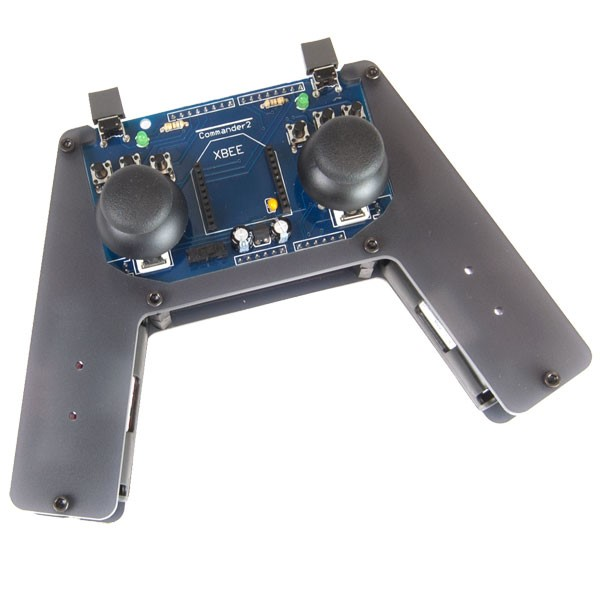
\includegraphics[scale=0.6]{./images/remote_controller}
			\caption{Remote controller}
		\end{figure}
		
		The robotic arm’s movements could be logged into files too and we could improve our code with the analysis of these files. That could be realised with a cheap SD card shield and with a very simple software module.
		
		\begin{figure}[H]
			\centering
			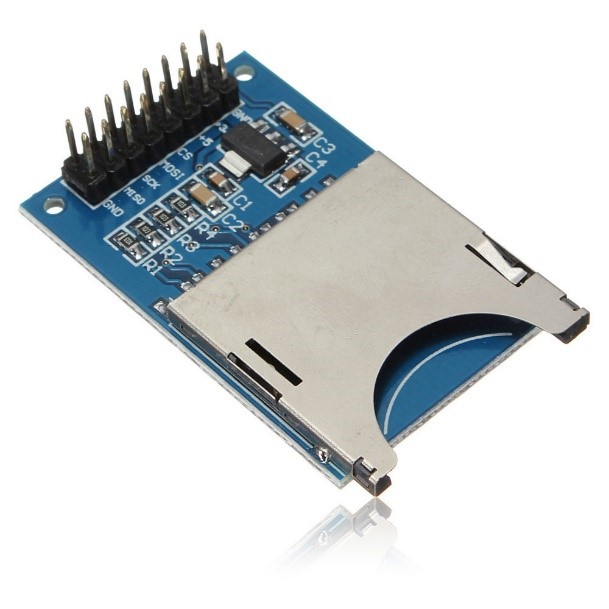
\includegraphics[scale=0.75]{./images/sd_card_shield}
			\caption{SD card shield}
		\end{figure}
		
		This hardware could be a part of an interesting co-robot system where we have to pay attention to the safety of the living workforce, or it can be mixed with a multiple manipulator system in which some steps are automated, some are done by human workforce.